\documentclass[12pt,]{article}
\usepackage[utf8]{inputenc}
\usepackage[T1]{fontenc}
\usepackage{mathptmx}
\usepackage{geometry}
\usepackage{mathtools}
\usepackage[english]{babel}
\usepackage{graphicx}
\usepackage{subcaption}
\usepackage{stackengine}
\usepackage[os=win]{menukeys}
\usepackage{hyperref}
\usepackage{minted}
\usepackage{xcolor}
\usepackage{tikz}
\usepackage[yyyymmdd,hhmmss]{datetime}
\usepackage{etoolbox}
\usepackage[inline]{enumitem}
\usepackage{pdfpages}

\newcommand{\WindowsLogo}{\raisebox{-0.1em}{
\includegraphics[height=0.8em]{images/logo/Windows_3_logo_simplified}}}
%\newcommand{\PowerLogo}{\raisebox{-0.1em}{
\includegraphics[height=0.8em]{images/logo/power}}}
\newcommand{\WinKey}{\keys{\WindowsLogo}}
\newcommand{\PowerKey}{\keys{\PowerLogo}}

\patchcmd{\thebibliography}{\section*{\refname}}{}{}{}

\newcommand{\ShowOsVersion}{
	\immediate\write18{\unexpanded{foo=`uname -sro` && echo "${foo}" > tmp.tex}}
	\input{tmp}\immediate\write18{rm tmp.tex}
}

\newcommand{\ShowTexVersion}{
	\immediate\write18{\unexpanded{foo=`pdflatex -version | head -n1 | cut -d' ' -f1,2` && echo "${foo}" > tmp.tex}}
	\input{tmp}\immediate\write18{rm tmp.tex}
}

\addto\captionsenglish{\renewcommand{\contentsname}{Daftar Isi}}
\addto\captionsenglish{\renewcommand{\figurename}{Gambar}}

\hypersetup{
	colorlinks=true, %set true if you want colored links
	linktoc=all,     %set to all if you want both sections and subsections linked
	linkcolor=blue,  %choose some color if you want links to stand out
	urlcolor=blue,   %url color
}

\geometry{
	a4paper,
	left=10mm,
	right=10mm,
	top=10mm,
	bottom=15mm,
}

\title{\LARGE \bf
	Laporan Pengujian Unit Prototype Handheld Audiometri (Tahap 1)\\
}

\author{Achmadi ST MT}

\date{}

\hypersetup{citecolor=black}

\definecolor{LightGray}{gray}{0.95}

%\pagecolor[rgb]{0.1,0.1,0.1}
%\color[rgb]{1,1,1}

\begin{document}
	\thispagestyle{empty}

	\begin{titlepage}
		\centering
		\vfill
		\vfill
		\maketitle
		\vfill
		
\includegraphics[width=200pt]{images/logo/logoviblab}
		\vfill
		\vfill
		Update: {\today} \currenttime \\
	\end{titlepage}

	%%%%%%%%%%%%%%%%%%%%%%%%%%%%%%%%%%%%%%%%%%%%%%%%%%%%%%%%%%%%%%%%%

	\newpage
	\tableofcontents

	%%%%%%%%%%%%%%%%%%%%%%%%%%%%%%%%%%%%%%%%%%%%%%%%%%%%%%%%%%%%%%%%%

	\newpage
	\section{Pendahuluan}

	\subsection{Tujuan Pengujian}

	Tujuan Pengujian disini adalah untuk mengetahui nilai aktual \textit{loudness} output dalam dB (SPL).

	\subsection{Waktu dan Tempat Pengujian}

	Seluruh pengujian di lakukan di Ruang Un-Echoic Chamber Laboratorium Fisika Bangunan Teknik Fisika
	Institut Teknologi Bandung. Waktu pengujian adalah minggu kedua di bulan Desember 2020.

	\subsection{Batasan Pengujian}

	Batasan pengujian adalah sebagai berikut:

	\begin{enumerate}
		\item Nilai frekuensi dan konsistensi frekuensi tidak diukur di ruang Unechoic chamber tersebut di atas
		karena telah diuji selama proses pengembangan dan perakitan unit prototype dan telah terbukti konsisten pada nilai yang diinginkan.

		\item Pengujian tidak dilakukan pada tubuh manusia sebenarnya melainkan menggunakan manekin yang diproduksi oleh GRASS KEMAR.
	\end{enumerate}

	%%%%%%%%%%%%%%%%%%%%%%%%%%%%%%%%%%%%%%%%%%%%%%%%%%%%%%%%%%%%%%%%%

	\newpage
	\section{Metode Pengujian}

	\subsection{Persiapan}

	Berikut adalah perangkat keras yang perlu disiapkan untuk pengujian ini:

	\begin{itemize}

		\item Unit Prototype Audiometri yang akan diuji.

		Pastikan unit prototype masih normal sebagaimana pada bab sebelumnya.

		\begin{figure}[!ht]
			\centering
			\begin{subfigure}[b]{0.3\textwidth}
				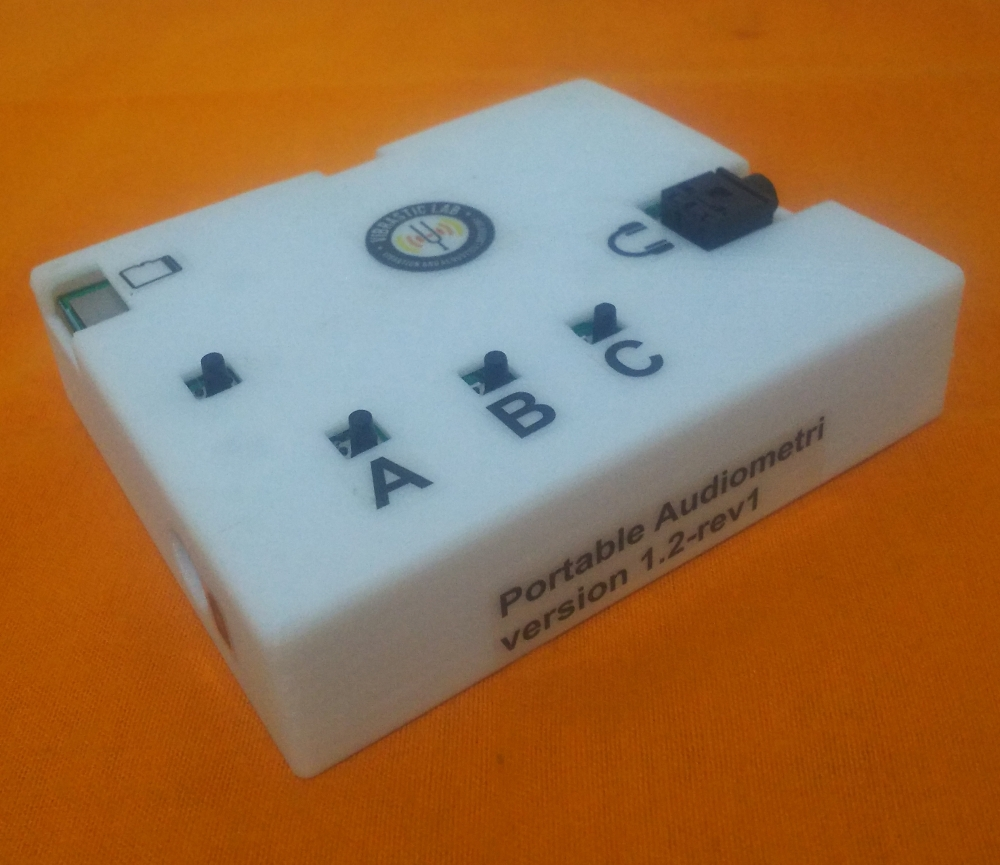
\includegraphics[width=\textwidth]{images/foto/unit}
				\caption{Unit Prototype}
			\end{subfigure}
			\begin{subfigure}[b]{0.3\textwidth}
				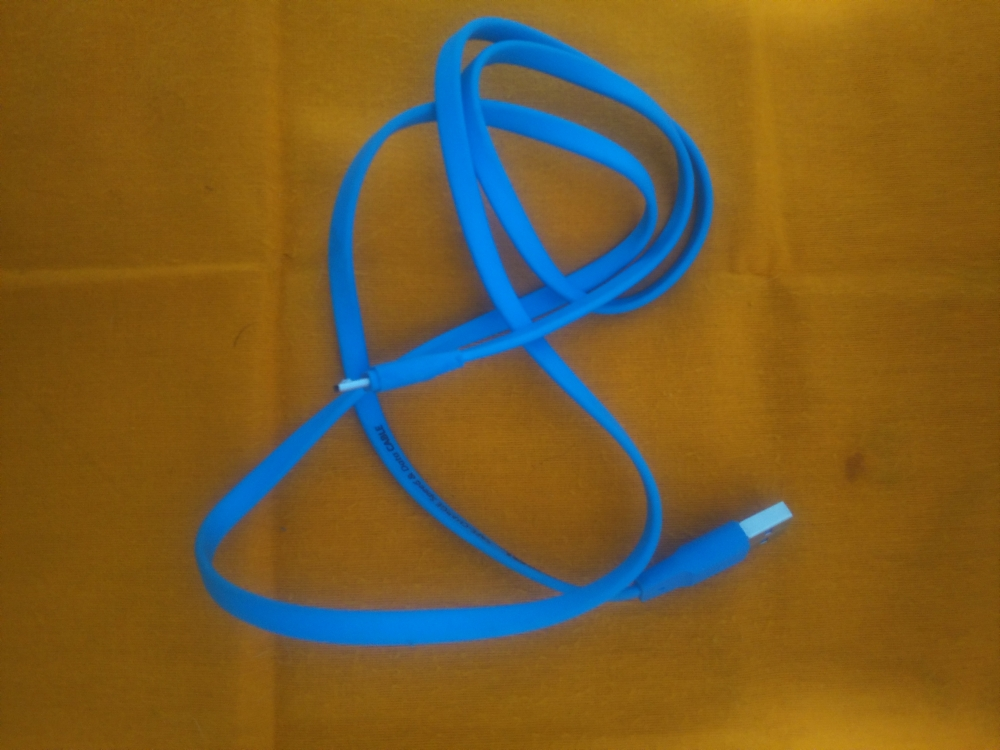
\includegraphics[width=\textwidth]{images/foto/kabel}
				\caption{Kabel USB}
			\end{subfigure}
			\caption{Prototype}
		\end{figure}


		\item Wired-Headphone dengan impedansi tiap channel antara $32\Omega$ hingga $300\Omega$

		Headphone yang digunakan disini adalah:
		\begin{itemize}
			\item Headphone Miniso (tanpa active noise cancelling)
			\item Headphone BOSE (dilengkapi active noise cancelling)
		\end{itemize}
		\begin{figure}[!ht]
			\centering
			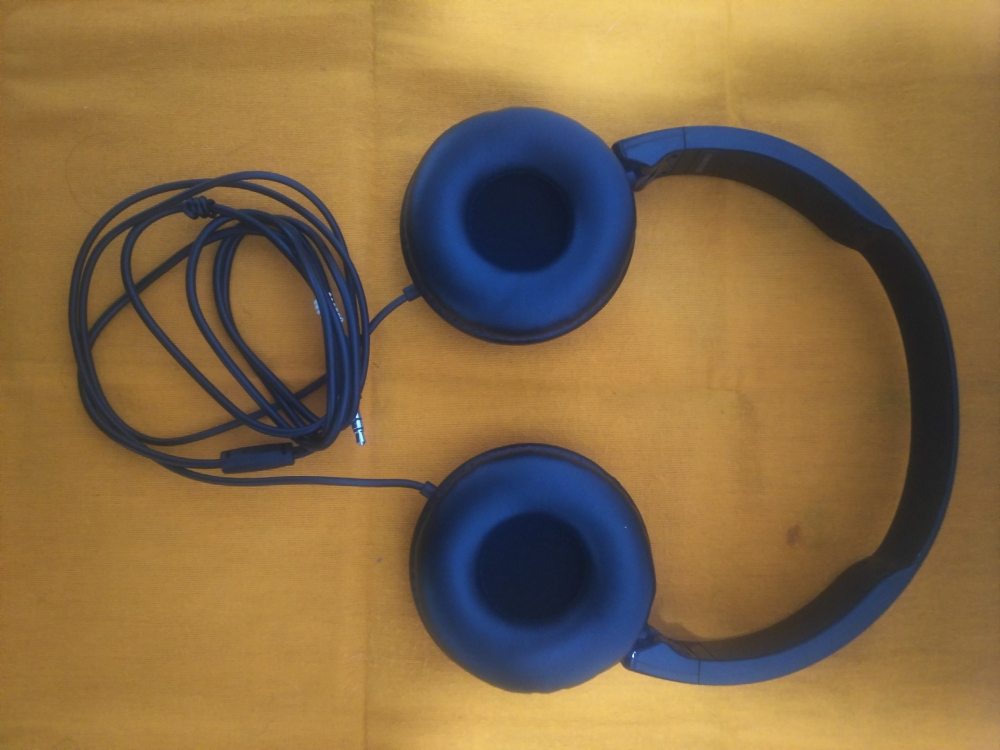
\includegraphics[width=200pt]{images/foto/phone}
			\caption{Wired Headphone}
		\end{figure}

		\newpage
		\item Kalibrasi Mikrofon pada manekin KEMAR menggunakan \textit{tone generator} yang tersedia pada paket GRASS KEMAR.
		Kemudian pasang Headphone pada manekin.
		\begin{figure}[!ht]
			\centering
			\begin{subfigure}[b]{0.3\textwidth}
				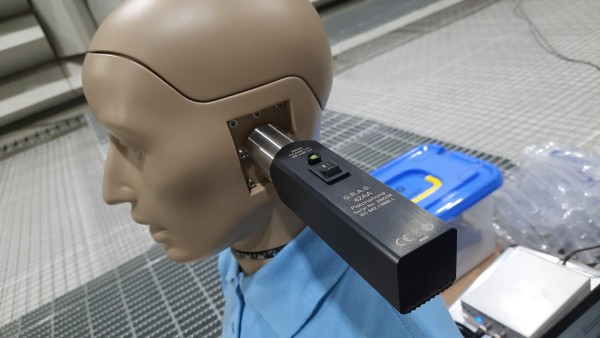
\includegraphics[width=\textwidth]{images/foto/calib}
				\caption{Kalibrasi Mikrofon}
			\end{subfigure}
			\begin{subfigure}[b]{0.3\textwidth}
				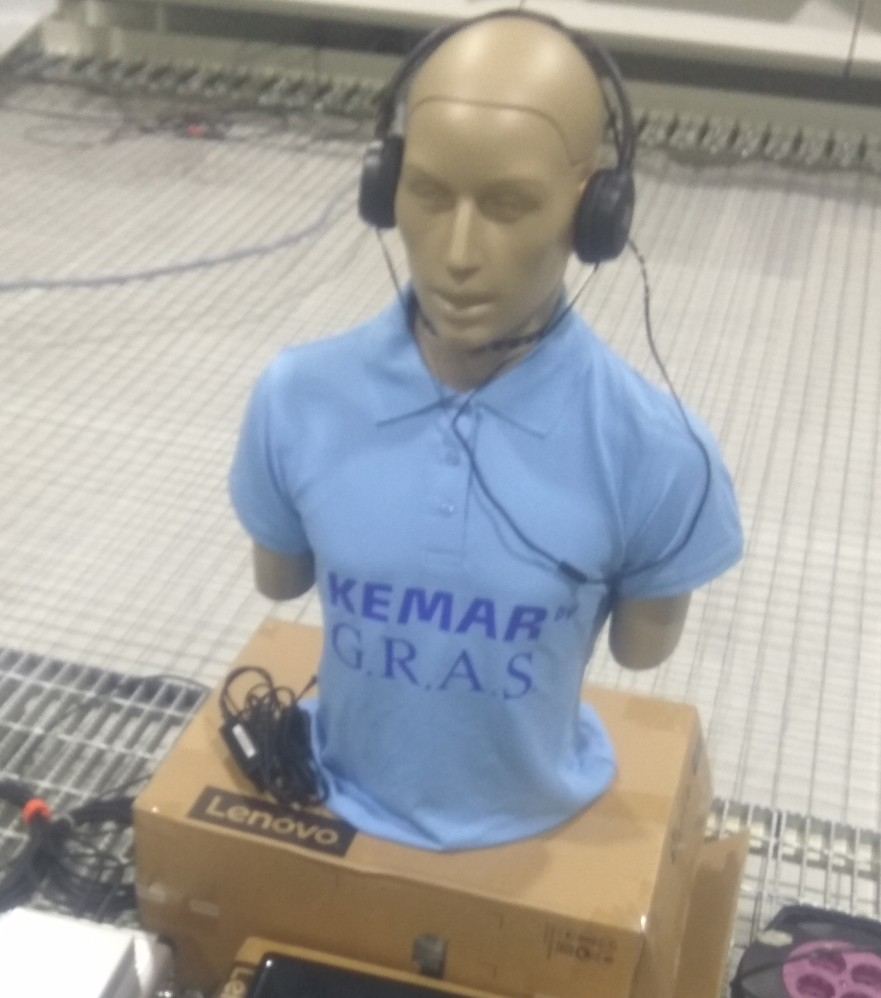
\includegraphics[width=\textwidth]{images/foto/kemar}
				\caption{Headphone Terpasang}
			\end{subfigure}
			\caption{GRASS KEMAR}
		\end{figure}

	\end{itemize}

	\subsection{Audio Analyzer}

	Mikrofon GRASS KEMAR dihubungkan dengan Audio-Box dan data Audio digital dikumpulkan dengan perangkat lunak Real-Time Analyzer via USB.
	Perangkat lunak ini merupakan bagian dari paket software DSFF3 buatan Yoshimasha.

	\begin{figure}[!ht]
		\centering
		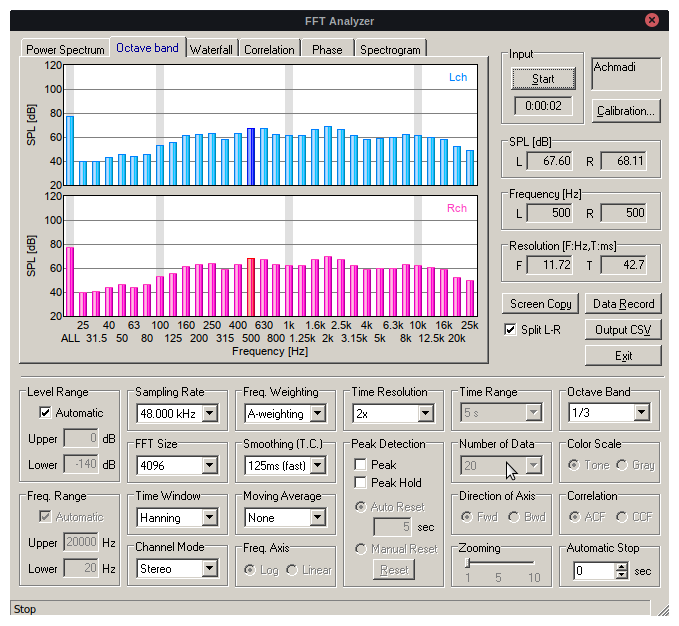
\includegraphics[width=300pt]{images/kemar/fft}
		\caption{Tampilan Audio Analyzer}
	\end{figure}

	\newpage
	\subsection{Teknis Pengujian}

	Berikut langkah proses pengujian

	\begin{itemize}
		\item Nyalakan unit prototype dan sambungkan USB protype ke komputer.
		\begin{figure}[!ht]
			\centering
			\begin{subfigure}[b]{0.3\textwidth}
				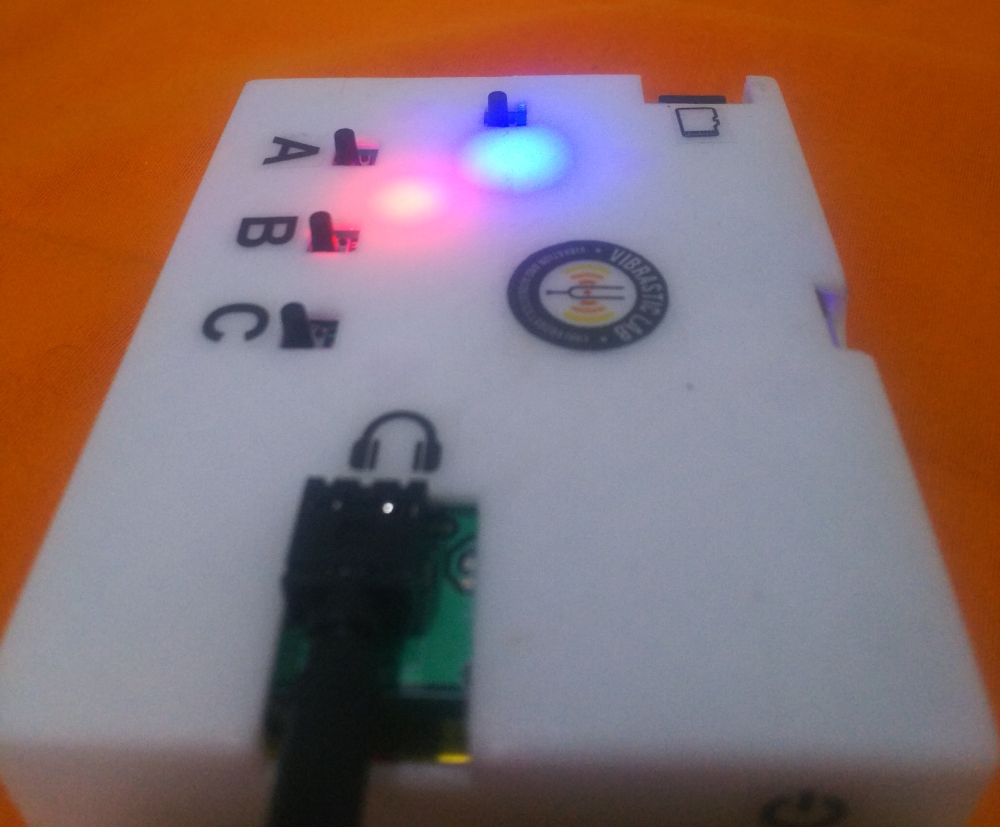
\includegraphics[width=\textwidth]{images/foto/standby}
				\caption{Prototype Standby}
			\end{subfigure}
			\begin{subfigure}[b]{0.3\textwidth}
				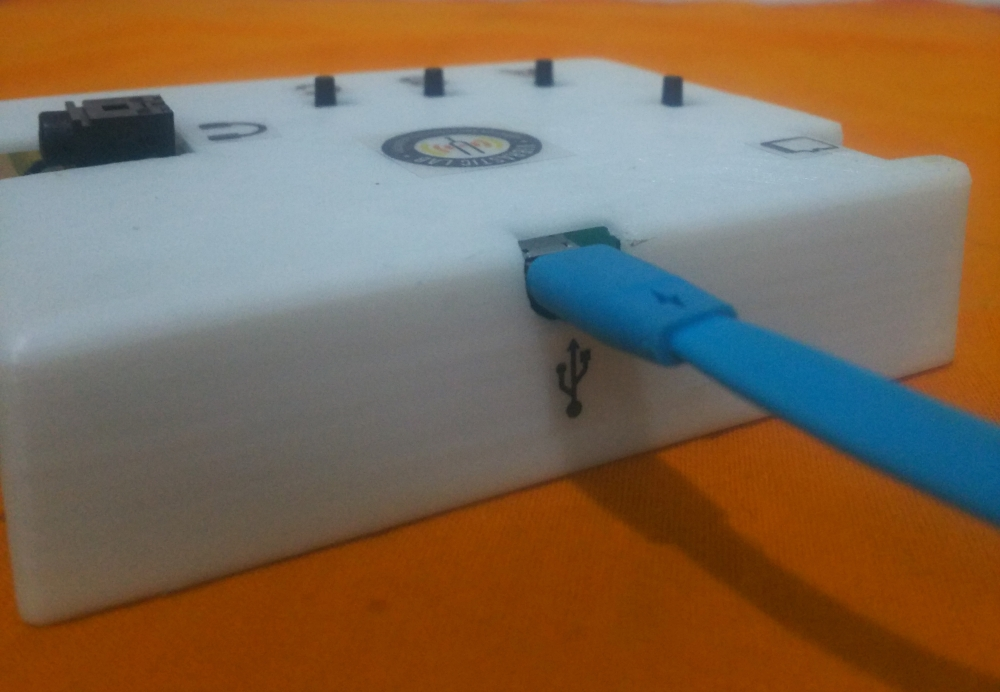
\includegraphics[width=\textwidth]{images/foto/konek}
				\caption{USB Terpasang}
			\end{subfigure}
			\caption{Menyalakan Unit Prototype}
		\end{figure}


		\item Akses prototype menggunakan serial port (semisal Hercules.exe) pada komputer.
		\begin{figure}[!ht]
			\centering
			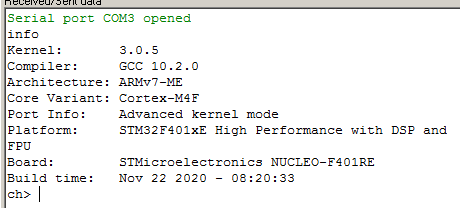
\includegraphics[width=300pt]{images/terminal/hercules_text}
			\caption{Contoh respon serial port}
		\end{figure}

		\item Perintah Serial untuk membangkitkan tone
		Perintah untuk membangkitkan tone dengan frekuensi dan skala yang diinginkan selama 5detik.

		Pola perintah serialnya adalah:
		\begin{minted}[frame=lines,framesep=2mm,fontsize=\small]{text}
out <frekuensi> <amplitudo>
		\end{minted}

		dengan:
		\begin{itemize}

			\item frekuensi adalah nilai frekuensi (dalam Hz) mulai 250, 500, 1000, 2000, 4000, dan 8000.

			\item amplitudo adalah skala amplitudo pada nilai 1, 2, 3, 4, 5, 6, 7, 8, dan 9.

		\end{itemize}

		Contoh untuk tone 500Hz pada skala amplitudo 6 (diakhiri (\keys{\return})):
		\begin{minted}[frame=lines,framesep=2mm,fontsize=\small]{text}
out 500 6
		\end{minted}

		\newpage
		Maka salah satu channel headphone yang terhubung prototype akan membangkitkan tone selama 5 detik.

		\begin{figure}[!ht]
			\centering
			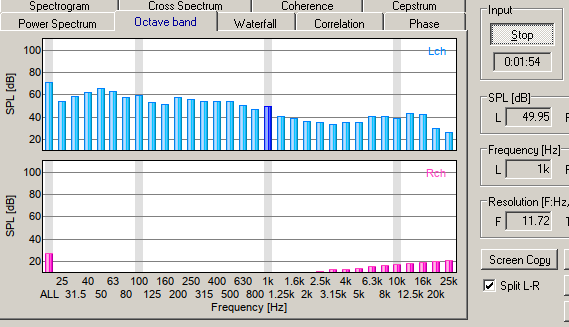
\includegraphics[width=300pt]{images/terminal/contoh}
			\caption{Contoh Nilai Uji}
		\end{figure}

		\item Hasil yang diinginkan adalah tabel dengan spesifikasi berikut:
		\begin{itemize}
			\item tabel loudness output di setiap frekuensi untuk setiap skala amplitudo, untuk 2 prototype dengan 2 headphone
			\item tabel loudness output di setiap frekuensi untuk setiap skala amplitudo, untuk 2 prototype dengan 2 headphone
		\end{itemize}

		sehingga diharapkan total 4 tabel hasil pengukuran.
	\end{itemize}

	\newpage
	\section{Hasil Pengujian}

	\subsection{Tabel Hasil}

	Tabel hasil pengujian cukuk banyak yang akan memakan tempat disini sehingga disediakan tempat di repository pemrograman Lab Vibrastic pada tautan berikut:\\
	\url{https://github.com/VibrasticLab/pikoakustik/tree/stm32f401re_3pin/document/hasil_ukur_lanjutan/tabel_hasil_ukur}.\\

	Kemudian untuk memudahkan proses pengolahan data, digunakan pula perangkat lunak Jupyter Note yang berkasnya dapat diakses di tautan:\\
	\url{https://github.com/VibrasticLab/pikoakustik/blob/stm32f401re_3pin/document/hasil_ukur_lanjutan/python/hasil_itb.ipynb}\\

	\subsection{Pengolahan Data}

	Pengolahan data hasil pengujian digunakan untuk mendapatkan model loudness.

		Dengan merata-rata matrix tabel didapat matrix untuk headphone Bose sebagai berikut:

		\[\left[
		\begin{matrix}
			34.4 & 36.5 & 40.7 & 45.7 & 51.4 & 57.4 & 63.4 & 69.5 & 75.6 \\
			32.6 & 35.8 & 40.2 & 44.9 & 50.2 & 56.6 & 62.7 & 68.8 & 74.8 \\
			37.7 & 41   & 45.5 & 51   & 56.8 & 62.9 & 69   & 75   & 81   \\
			36.3 & 38.6 & 42.4 & 47.7 & 53.2 & 59.2 & 65.4 & 71.4 & 77.4 \\
			41.1 & 43.8 & 48   & 53.2 & 59   & 64.9 & 71.1 & 77.1 & 83.1 \\
			41.8 & 42.6 & 44.9 & 49   & 54.4 & 60.2 & 66.2 & 72.2 & 78.2 \\
		\end{matrix}
		\right]\]

		Pendekatan model matematis untuk loudness terhadap skala input menggunakan polynomial:\\
		\[f(x) = ax^3 + bx^2 + cx + d\]

		Estimasi model menggunakan perangkat lunak Numpy Polyfit yang tersedia di Python.
		Hasil estimasi untuk headphone Bose pada setiap frekuensi.

		\[f_{250}(x) = 0.05x^3 - 0.46x^2 - 4.7x + 80.5\]
		\[f_{500}(x) = 0.03x^3 - 0.28x^2 - 5.4x + 80.48\]
		\[f_{1000}(x) = 0.04x^3 - 0.4x^2 - 4.8x + 86.06\]
		\[f_{2000}(x) = 0.05x^3 - 0.49x^2 - 4.59x + 82.33\]
		\[f_{4000}(x) = 0.04x^3 - 0.44x^2 - 4.72x + 88.12\]
		\[f_{8000}(x) = 0.06x^3 - 0.59x^2 - 4.37x + 83\]

		Model matematis ini yang akan di implementasikan ke prototype.

		Selanjutnya untuk headphone Miniso, dilakukan metode perhitungan yang sama.

		Berikut matrix rata-rata loudness pengukuran:

		\[\left[
		\begin{matrix}
			36   & 39.5 & 44.2 & 49.7 & 55.6 & 61.4 & 67.4 & 73.4 & 79.4 \\
			36.7 & 40.5 & 45.4 & 50.8 & 56.7 & 62.6 & 68.6 & 74.6 & 80.6 \\
			39.9 & 43.6 & 48.6 & 54.2 & 60   & 65.9 & 71.8 & 77.8 & 83.8 \\
			33   & 35.4 & 39.6 & 44.7 & 50.4 & 56.4 & 62.4 & 68.3 & 74.4 \\
			32.7 & 33.4 & 35.3 & 39.2 & 44.3 & 50   & 56   & 62   & 68   \\
			35.6 & 36.2 & 38.3 & 41.8 & 47   & 52.6 & 58.6 & 64.6 & 70.5 \\
		\end{matrix}
		\right]\]

		Hasil estimasi untuk Headphone Miniso pada setiap frekuensi.

		\[f_{250}(x) = 0.03x^3 - 0.32x^2 - 4.99x + 84.58\]
		\[f_{500}(x) = 0.03x^3 - 0.28x^2 - 5.16x + 85.93\]
		\[f_{1000}(x) = 0.03x^3 - 0.28x^2 - 5.09x + 36.38\]
		\[f_{2000}(x) = 0.04x^3 - 0.46x^2 - 4.63x + 37.21\]
		\[f_{4000}(x) = 0.06x^3 - 0.53x^2 - 4.64x + 39.77\]
		\[f_{8000}(x) = 0.06x^3 - 0.51x^2 - 4.67x + 42.73\]

	\newpage
	\section{Lampiran}

	\subsection{Notebook Olah Data}
	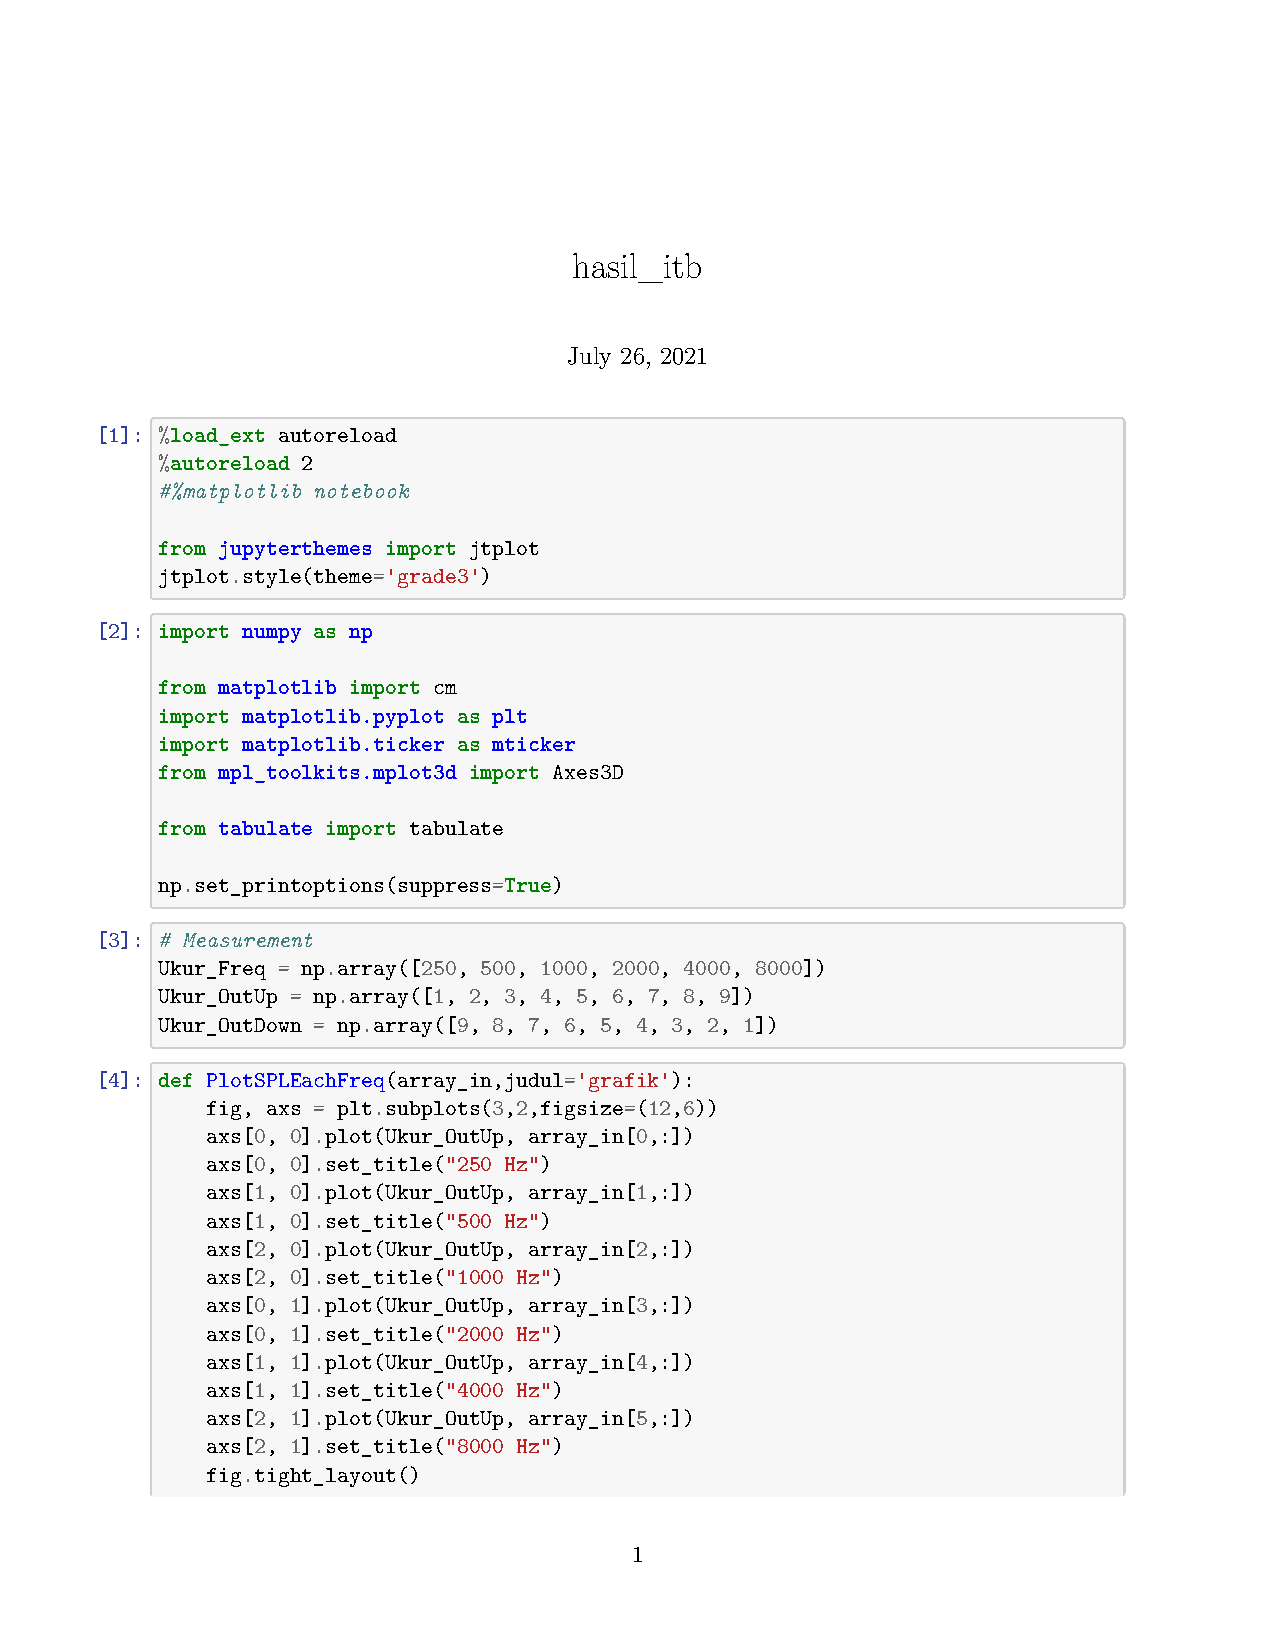
\includepdf[pages=-]{python/hasil_itb.pdf}

\end{document}
